	\chapter{Action start merge -as}
	Suppose we have action $a$ that can be executed in init and can be executed at most once. Such action holds an invariant effect of type $<u_i,u_j>$ where $u_j$ is not used in any other action. But if we know that $a$ has invariant effect $<u_i,u_j>$ and also effect $<w_i,w_j>$ so then, there could be invariant effect $<w_j,w_i>$ in other actions. If there are such a link, then action $a$ is applied - this is what this operation does.
	
	But in implementation (as in older text here) are some mistakes. Firstly, $a$ can have prevails preconditions but they have to be satisfied by init.
	
	\textbf{Another mistake} written here and already implemented is that there is no check whether action $a$ does not destroy usage of other actions. So, there should be or - either effect in $a$ in the is invariant, invariant together with another action (there is the cycle) or it deletes something that is not used in any other function (not in delete effect nor prevail preconditions).
	
	Also, this operation seems to be old, because after implementing -sf, -ai, -ou and -oe these reduction may have the same effect as this one. Suppose that firstly -ou removes replaces invariant by new one (by adding new fact), then if -ai or -sf is applied, the action $a$ can be merged with start.
	
	\begin{figure}
		\begin{subfigure}[b]{0.4\textwidth}
			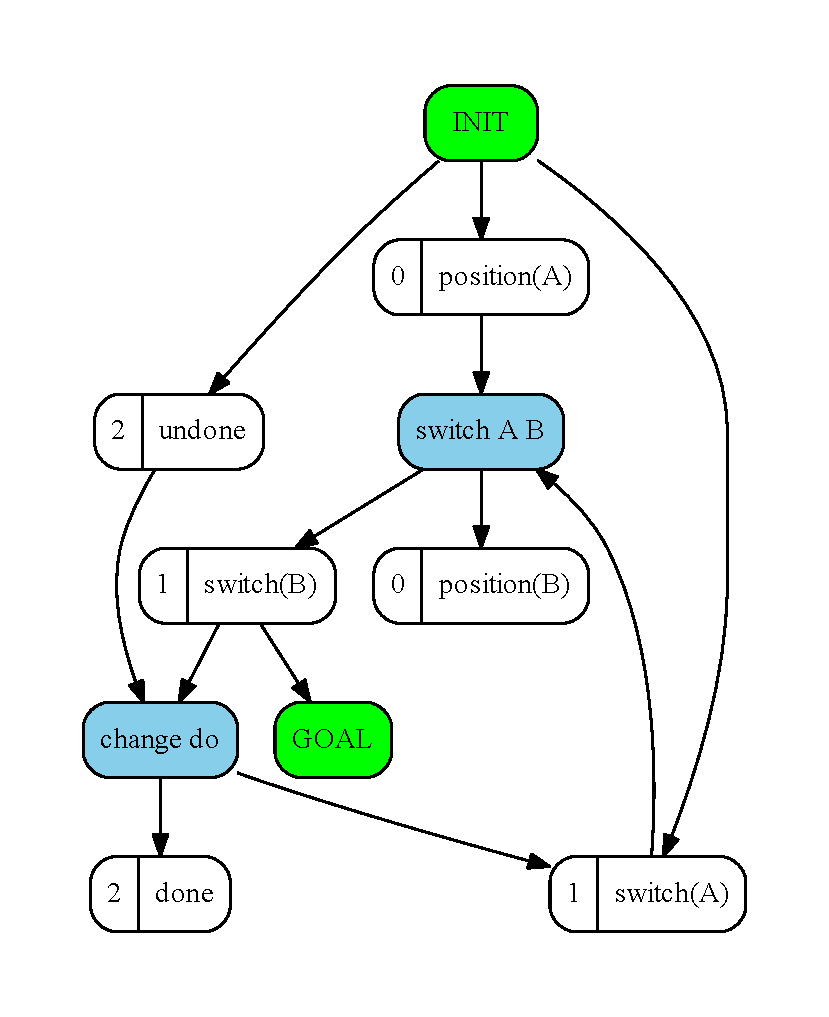
\includegraphics[scale=0.4]{actionStartMerge/figures/simple_input}
			\caption{before reduction}
		\end{subfigure}	
		\begin{subfigure}[b]{0.4\textwidth}
			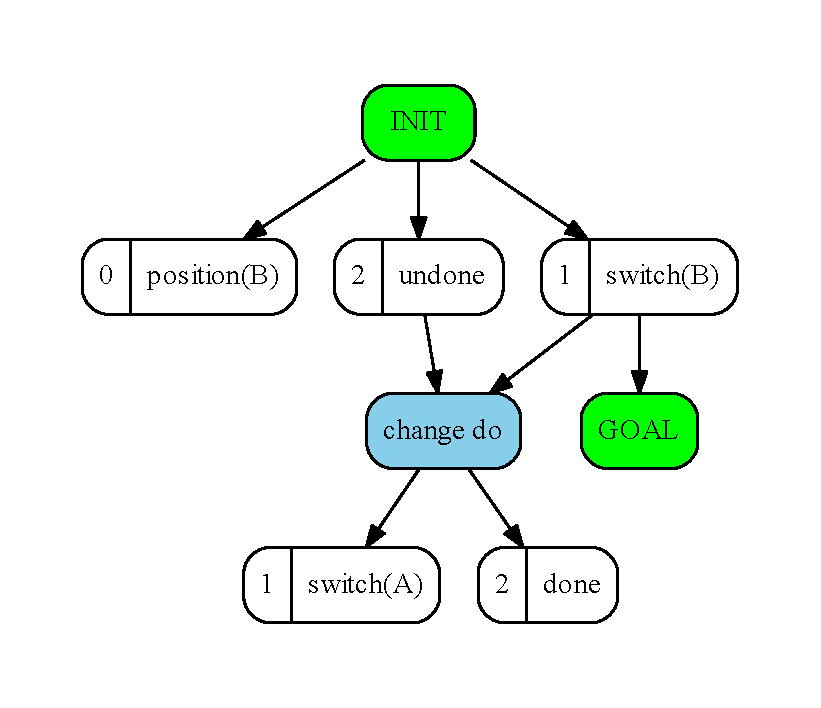
\includegraphics[scale=0.4]{actionStartMerge/figures/simple_output}
			\caption{after reduction}
		\end{subfigure}
		\caption{Action \emph{switch A B} was applied because it is applicable in init, it can be used at most once ($<\emph{0 position(A), 0 position(B)}>$). Since this action can be applied at most once, then \emph{change do} can be also applied at most once. So, \emph{switch A B} can be merged with start because it will not destroy application of any other function.	}
	\end{figure}
	
	\section{Reduce operation}
	Let's have SAS in form $<\vars, \init, \goal, \actions, \mutexes{}>$. There must be following values and actions in order to execute the action:
	
	\begin{enumerate}
		\item $a \in \actions$
		\item $|\pre{a}| = 0$ - such is implementation, $\pre{a} \subseteq{\init}$ is better 
		\item $<u_i,u_j> \in \eff{a}$
		\item $u_i \in \init$, $|\con{u_i}| = 1$
		\item $|\con{u_j}| = 0$
		\item $\forall <w_i, w_j> \in \eff{a}, \var{w_i} \neq \var{v_i}:$
		\begin{itemize}
			\item $w_i \in \init$
			\item $ \forall a_p \in \pro{w_i}: <w_j,w_i> \in a_p $ 
			\item $ \forall a_c \in \con{w_j}: <w_j,w_i> \in a_c $ 
		\end{itemize}
	\end{enumerate}
	
	Such effect $<u_i, u_j>$ with condition over $u_i$ and $u_j$ ensures that $a$ can be executed only once and in init. For each different effect than $<u_i,u_j>$, let say $<w_i,w_j>$, there must hold that all action consuming $w_j$ also contains effect $<w_j,w_i>$ and that there are only one action that needs $w_i$ (action $a$).
	
	The operation does following things:
	
	\begin{enumerate}
		\item for each effect $e \in \eff{a}$, $e = <w_i, w_j>$; do: $u_i$ is replaced by $u_j$ in $\init$, $u_i$ is replaced by $u_j$ in mutexes and in init
		\item remove $u_i$ from $\dom{\var{u_i}}$
		\item final init is stored in $\init{}'$
		\item $\actions{}' \leftarrow \actions \setminus \{a\}$
		\item for each effect $<w_i,w_j> \in \eff{a}, \var{w_i} \neq \var{u_i}$ do following things
		\begin{enumerate}
			\item $\actions{}'  \leftarrow \actions$
			\item for each $a_p \in \pro{w_i} \cup \con{w_j}$ do following
			\item $a_n \leftarrow <\pre{a_p} \cup{w_j}, \eff{a_p} \setminus \{<w_i,w_j>,<w_j,w_i>\} >$
			\item if $|\eff{a_p}| > 0$ $\actions{}' \leftarrow (\actions{}' \setminus \{a_p\}) \cup \{a_n\}$
			\item else $\actions{}' \leftarrow \actions{}' \setminus \{a_p\}$ 
		\end{enumerate}
	\end{enumerate}
	
	Output of the reduction is SAS $<\vars{}', \init{}', \goal{}, \actions{}', \mutexes{}'>$.
	
	
	\section{Possible outgoing states of SAS}
	\begin{enumerate}
		\item possible empty mutex
		\item possible state of SAS for delete variable -dv, merging actions -mo, simple dependency -sd, maybe even one usage reduction -ou and action start merge -as, -sf, -ai
	\end{enumerate}
	
	\section{States before application of this operation}
	\begin{itemize}
		\item SAS from beginning
		\item after -mo, -ou, -dv
		\item maybe after -oe, -as, -ai, -sf
	\end{itemize}
	
	
	\section{Reverse operation}
	Removed actions and values are added back and added actions $a_n$ are removed from the action set. Action $a$ is added at the first position in the plan and such extended plan is returned.
	
	\section{Implementation notes}
	Simple implementation without any advance caching. There may be speed up by comparing set $\con{w_j} = \pro{w_i}$, if they equal. Now, the implementation is done as written above - for each effect, it check if all consumers and producers have got the right effect.
	
	
	